\documentclass[twoside]{book}

% Packages required by doxygen
\usepackage{fixltx2e}
\usepackage{calc}
\usepackage{doxygen}
\usepackage[export]{adjustbox} % also loads graphicx
\usepackage{graphicx}
\usepackage[utf8]{inputenc}
\usepackage{makeidx}
\usepackage{multicol}
\usepackage{multirow}
\PassOptionsToPackage{warn}{textcomp}
\usepackage{textcomp}
\usepackage[nointegrals]{wasysym}
\usepackage[table]{xcolor}

% Font selection
\usepackage[T1]{fontenc}
\usepackage[scaled=.90]{helvet}
\usepackage{courier}
\usepackage{amssymb}
\usepackage{sectsty}
\renewcommand{\familydefault}{\sfdefault}
\allsectionsfont{%
  \fontseries{bc}\selectfont%
  \color{darkgray}%
}
\renewcommand{\DoxyLabelFont}{%
  \fontseries{bc}\selectfont%
  \color{darkgray}%
}
\newcommand{\+}{\discretionary{\mbox{\scriptsize$\hookleftarrow$}}{}{}}

% Page & text layout
\usepackage{geometry}
\geometry{%
  a4paper,%
  top=2.5cm,%
  bottom=2.5cm,%
  left=2.5cm,%
  right=2.5cm%
}
\tolerance=750
\hfuzz=15pt
\hbadness=750
\setlength{\emergencystretch}{15pt}
\setlength{\parindent}{0cm}
\setlength{\parskip}{0.2cm}
\makeatletter
\renewcommand{\paragraph}{%
  \@startsection{paragraph}{4}{0ex}{-1.0ex}{1.0ex}{%
    \normalfont\normalsize\bfseries\SS@parafont%
  }%
}
\renewcommand{\subparagraph}{%
  \@startsection{subparagraph}{5}{0ex}{-1.0ex}{1.0ex}{%
    \normalfont\normalsize\bfseries\SS@subparafont%
  }%
}
\makeatother

% Headers & footers
\usepackage{fancyhdr}
\pagestyle{fancyplain}
\fancyhead[LE]{\fancyplain{}{\bfseries\thepage}}
\fancyhead[CE]{\fancyplain{}{}}
\fancyhead[RE]{\fancyplain{}{\bfseries\leftmark}}
\fancyhead[LO]{\fancyplain{}{\bfseries\rightmark}}
\fancyhead[CO]{\fancyplain{}{}}
\fancyhead[RO]{\fancyplain{}{\bfseries\thepage}}
\fancyfoot[LE]{\fancyplain{}{}}
\fancyfoot[CE]{\fancyplain{}{}}
\fancyfoot[RE]{\fancyplain{}{\bfseries\scriptsize Generated on Fri Sep 11 2015 18\+:43\+:19 for My Project by Doxygen }}
\fancyfoot[LO]{\fancyplain{}{\bfseries\scriptsize Generated on Fri Sep 11 2015 18\+:43\+:19 for My Project by Doxygen }}
\fancyfoot[CO]{\fancyplain{}{}}
\fancyfoot[RO]{\fancyplain{}{}}
\renewcommand{\footrulewidth}{0.4pt}
\renewcommand{\chaptermark}[1]{%
  \markboth{#1}{}%
}
\renewcommand{\sectionmark}[1]{%
  \markright{\thesection\ #1}%
}

% Indices & bibliography
\usepackage{natbib}
\usepackage[titles]{tocloft}
\setcounter{tocdepth}{3}
\setcounter{secnumdepth}{5}
\makeindex

% Hyperlinks (required, but should be loaded last)
\usepackage{ifpdf}
\ifpdf
  \usepackage[pdftex,pagebackref=true]{hyperref}
\else
  \usepackage[ps2pdf,pagebackref=true]{hyperref}
\fi
\hypersetup{%
  colorlinks=true,%
  linkcolor=blue,%
  citecolor=blue,%
  unicode%
}

% Custom commands
\newcommand{\clearemptydoublepage}{%
  \newpage{\pagestyle{empty}\cleardoublepage}%
}


%===== C O N T E N T S =====

\begin{document}

% Titlepage & ToC
\hypersetup{pageanchor=false,
             bookmarks=true,
             bookmarksnumbered=true,
             pdfencoding=unicode
            }
\pagenumbering{roman}
\begin{titlepage}
\vspace*{7cm}
\begin{center}%
{\Large My Project }\\
\vspace*{1cm}
{\large Generated by Doxygen 1.8.10}\\
\vspace*{0.5cm}
{\small Fri Sep 11 2015 18:43:19}\\
\end{center}
\end{titlepage}
\clearemptydoublepage
\tableofcontents
\clearemptydoublepage
\pagenumbering{arabic}
\hypersetup{pageanchor=true}

%--- Begin generated contents ---
\chapter{Hierarchical Index}
\section{Class Hierarchy}
This inheritance list is sorted roughly, but not completely, alphabetically\+:\begin{DoxyCompactList}
\item \contentsline{section}{Car}{\pageref{class_car}}{}
\begin{DoxyCompactList}
\item \contentsline{section}{Small\+Car}{\pageref{interface_small_car}}{}
\end{DoxyCompactList}
\item \contentsline{section}{Car()}{\pageref{category_car_07_08}}{}
\item N\+S\+Object\begin{DoxyCompactList}
\item \contentsline{section}{Math\+A\+P\+I}{\pageref{interface_math_a_p_i}}{}
\end{DoxyCompactList}
\item $<$U\+I\+Application\+Delegate$>$\begin{DoxyCompactList}
\item \contentsline{section}{App\+Delegate}{\pageref{interface_app_delegate}}{}
\end{DoxyCompactList}
\item U\+I\+Responder\begin{DoxyCompactList}
\item \contentsline{section}{App\+Delegate}{\pageref{interface_app_delegate}}{}
\end{DoxyCompactList}
\item U\+I\+View\+Controller\begin{DoxyCompactList}
\item \contentsline{section}{View\+Controller}{\pageref{interface_view_controller}}{}
\end{DoxyCompactList}
\item \contentsline{section}{View\+Controller()}{\pageref{category_view_controller_07_08}}{}
\end{DoxyCompactList}

\chapter{Class Index}
\section{Class List}
Here are the classes, structs, unions and interfaces with brief descriptions\+:\begin{DoxyCompactList}
\item\contentsline{section}{\hyperlink{interface_app_delegate}{App\+Delegate} }{\pageref{dd/d52/interface_app_delegate}}{}
\item\contentsline{section}{\hyperlink{class_car}{Car} }{\pageref{d6/d44/class_car}}{}
\item\contentsline{section}{\hyperlink{category_car_07_08}{Car()} }{\pageref{d1/d89/category_car_07_08}}{}
\item\contentsline{section}{\hyperlink{interface_math_a_p_i}{Math\+A\+P\+I} }{\pageref{df/d7d/interface_math_a_p_i}}{}
\item\contentsline{section}{\hyperlink{interface_small_car}{Small\+Car} }{\pageref{de/dcf/interface_small_car}}{}
\item\contentsline{section}{\hyperlink{interface_view_controller}{View\+Controller} }{\pageref{d2/d60/interface_view_controller}}{}
\item\contentsline{section}{\hyperlink{category_view_controller_07_08}{View\+Controller()} }{\pageref{d9/dee/category_view_controller_07_08}}{}
\end{DoxyCompactList}

\chapter{Class Documentation}
\hypertarget{interface_app_delegate}{}\section{App\+Delegate Class Reference}
\label{interface_app_delegate}\index{App\+Delegate@{App\+Delegate}}
Inheritance diagram for App\+Delegate\+:\begin{figure}[H]
\begin{center}
\leavevmode
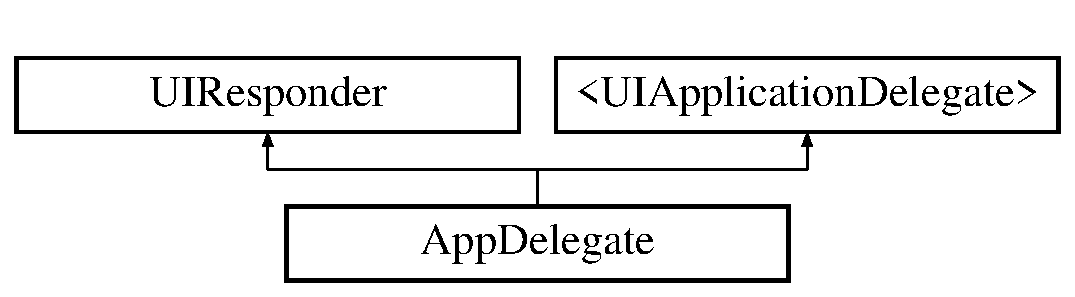
\includegraphics[height=2.000000cm]{dd/d52/interface_app_delegate}
\end{center}
\end{figure}
\subsection*{Properties}
\begin{DoxyCompactItemize}
\item 
\hypertarget{interface_app_delegate_acf48ac24125e688cac1a85445cd7fac2}{}U\+I\+Window $\ast$ {\bfseries window}\label{interface_app_delegate_acf48ac24125e688cac1a85445cd7fac2}

\end{DoxyCompactItemize}


The documentation for this class was generated from the following file\+:\begin{DoxyCompactItemize}
\item 
Documentation\+Examples/App\+Delegate.\+h\end{DoxyCompactItemize}

\hypertarget{class_car}{}\section{Car Class Reference}
\label{class_car}\index{Car@{Car}}
Inheritance diagram for Car\+:\begin{figure}[H]
\begin{center}
\leavevmode
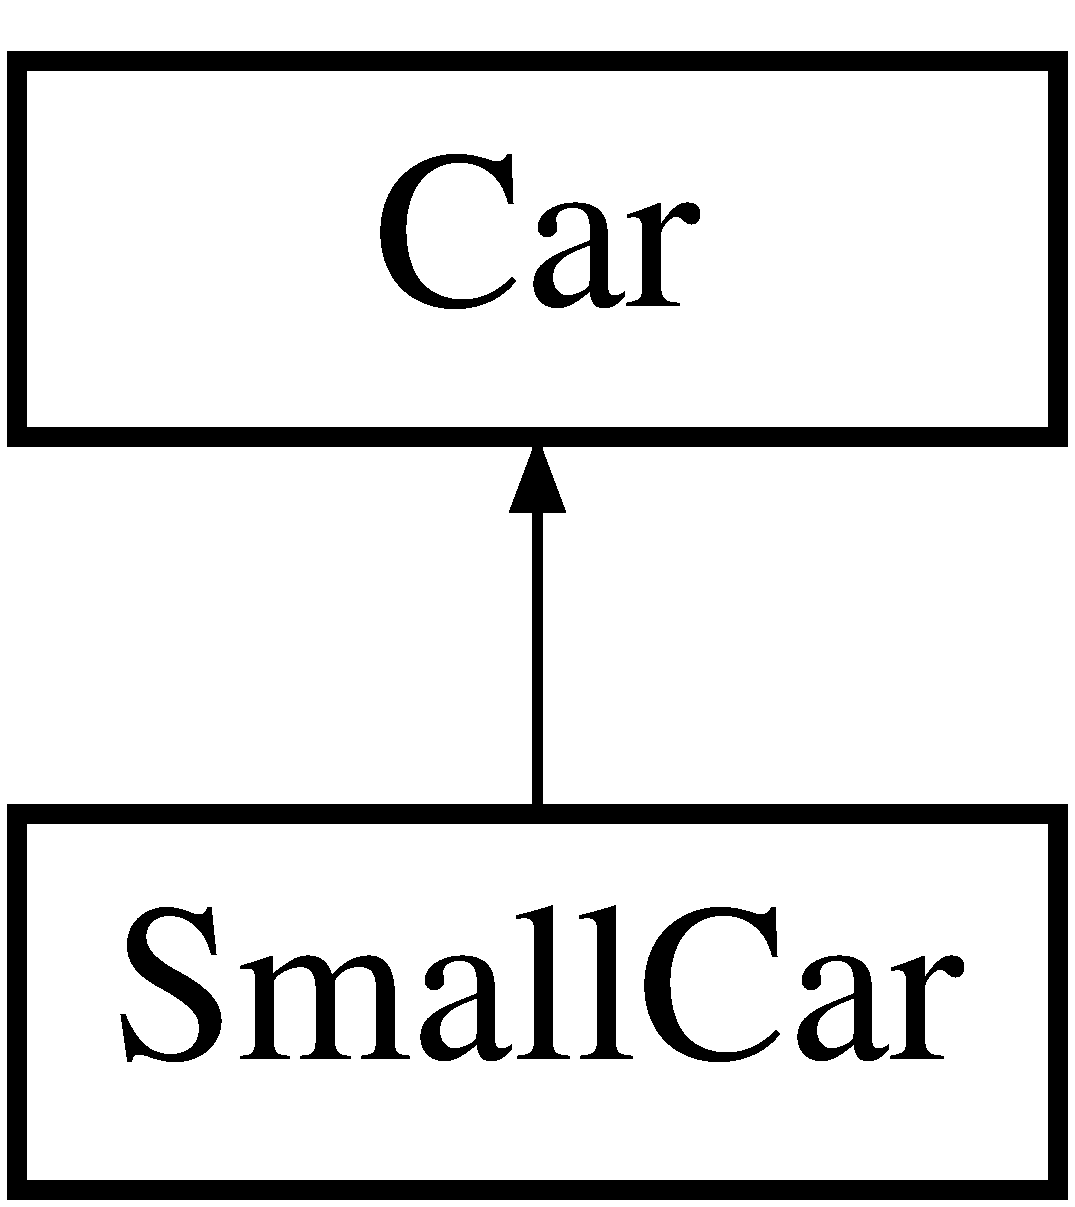
\includegraphics[height=2.000000cm]{d6/d44/class_car}
\end{center}
\end{figure}


The documentation for this class was generated from the following file\+:\begin{DoxyCompactItemize}
\item 
Documentation\+Examples/Car.\+m\end{DoxyCompactItemize}

\hypertarget{category_car_07_08}{}\section{Car() Category Reference}
\label{category_car_07_08}\index{Car()@{Car()}}
\subsection*{Properties}
\begin{DoxyCompactItemize}
\item 
\hypertarget{category_car_07_08_a2d6e4a02390f7c55946ced5318b3a4b2}{}C\+G\+Float {\bfseries distance\+Driven}\label{category_car_07_08_a2d6e4a02390f7c55946ced5318b3a4b2}

\end{DoxyCompactItemize}


The documentation for this category was generated from the following file\+:\begin{DoxyCompactItemize}
\item 
Documentation\+Examples/Car.\+m\end{DoxyCompactItemize}

\hypertarget{interface_math_a_p_i}{}\section{Math\+A\+P\+I Class Reference}
\label{interface_math_a_p_i}\index{Math\+A\+P\+I@{Math\+A\+P\+I}}
Inheritance diagram for Math\+A\+P\+I\+:\begin{figure}[H]
\begin{center}
\leavevmode
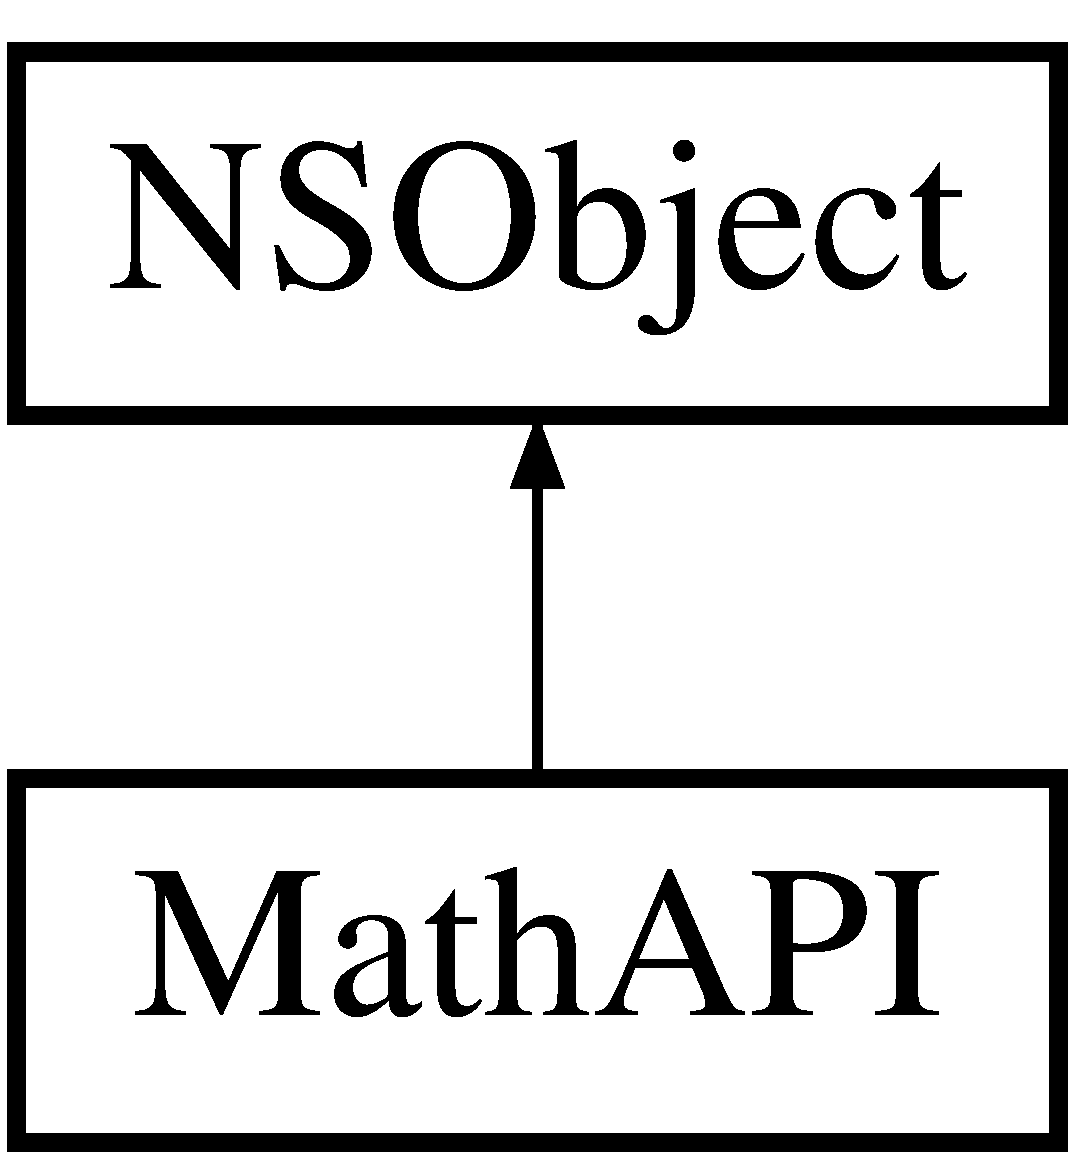
\includegraphics[height=2.000000cm]{df/d7d/interface_math_a_p_i}
\end{center}
\end{figure}
\subsection*{Class Methods}
\begin{DoxyCompactItemize}
\item 
(N\+S\+Integer) + \hyperlink{interface_math_a_p_i_a1cb98c1df6761206a09c65ffdb1d6cc1}{add\+Number\+:to\+Number\+:}
\end{DoxyCompactItemize}


\subsection{Method Documentation}
\hypertarget{interface_math_a_p_i_a1cb98c1df6761206a09c65ffdb1d6cc1}{}\index{Math\+A\+P\+I@{Math\+A\+P\+I}!add\+Number\+:to\+Number\+:@{add\+Number\+:to\+Number\+:}}
\index{add\+Number\+:to\+Number\+:@{add\+Number\+:to\+Number\+:}!Math\+A\+P\+I@{Math\+A\+P\+I}}
\subsubsection[{add\+Number\+:to\+Number\+:(\+N\+S\+Integer first\+Number,[to\+Number] N\+S\+Integer second\+Number)}]{\setlength{\rightskip}{0pt plus 5cm}+ (N\+S\+Integer) add\+Number\+: 
\begin{DoxyParamCaption}
\item[{(N\+S\+Integer)}]{first\+Number}
\item[{toNumber:(N\+S\+Integer)}]{second\+Number}
\end{DoxyParamCaption}
}\label{interface_math_a_p_i_a1cb98c1df6761206a09c65ffdb1d6cc1}
A really simple way to calculate the sum of two numbers.


\begin{DoxyParams}{Parameters}
{\em first\+Number} & An N\+S\+Integer to be used in the summation of two numbers \\
\hline
{\em second\+Number} & The second half of the equation. \\
\hline
\end{DoxyParams}
\begin{DoxyWarning}{Warning}
Please make note that this method is only good for adding non-\/negative numbers.
\end{DoxyWarning}
\begin{DoxyReturn}{Returns}
The sum of the two numbers passed in. 
\end{DoxyReturn}


The documentation for this class was generated from the following files\+:\begin{DoxyCompactItemize}
\item 
Documentation\+Examples/Math\+A\+P\+I.\+h\item 
Documentation\+Examples/Math\+A\+P\+I.\+m\end{DoxyCompactItemize}

\hypertarget{interface_small_car}{}\section{Small\+Car Class Reference}
\label{interface_small_car}\index{Small\+Car@{Small\+Car}}
Inheritance diagram for Small\+Car\+:\begin{figure}[H]
\begin{center}
\leavevmode
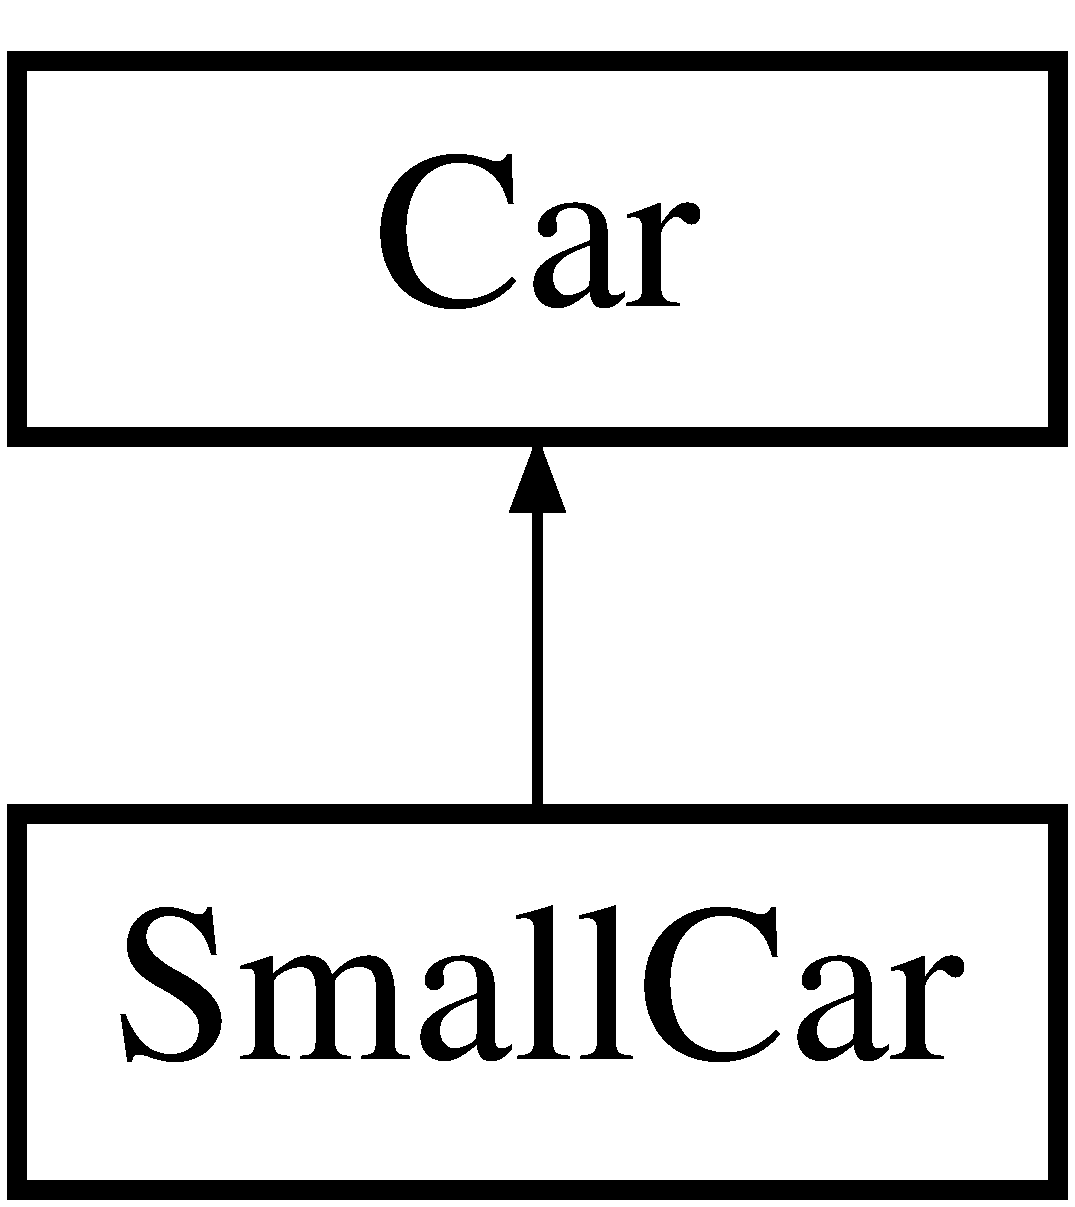
\includegraphics[height=2.000000cm]{interface_small_car}
\end{center}
\end{figure}
\subsection*{Properties}
\begin{DoxyCompactItemize}
\item 
U\+I\+Color $\ast$ \hyperlink{interface_small_car_a286abaea6871cde85bacc2e47fc31919}{exterior\+Color}
\item 
N\+S\+String $\ast$ \hyperlink{interface_small_car_ad1033f82517211f319f7b32ca0008f9a}{nickname}
\end{DoxyCompactItemize}


\subsection{Property Documentation}
\hypertarget{interface_small_car_a286abaea6871cde85bacc2e47fc31919}{}\index{Small\+Car@{Small\+Car}!exterior\+Color@{exterior\+Color}}
\index{exterior\+Color@{exterior\+Color}!Small\+Car@{Small\+Car}}
\subsubsection[{exterior\+Color}]{\setlength{\rightskip}{0pt plus 5cm}-\/ (U\+I\+Color$\ast$) exterior\+Color\hspace{0.3cm}{\ttfamily [read]}, {\ttfamily [write]}, {\ttfamily [nonatomic]}, {\ttfamily [assign]}}\label{interface_small_car_a286abaea6871cde85bacc2e47fc31919}
sub class comment test \hypertarget{interface_small_car_ad1033f82517211f319f7b32ca0008f9a}{}\index{Small\+Car@{Small\+Car}!nickname@{nickname}}
\index{nickname@{nickname}!Small\+Car@{Small\+Car}}
\subsubsection[{nickname}]{\setlength{\rightskip}{0pt plus 5cm}-\/ (N\+S\+String$\ast$) nickname\hspace{0.3cm}{\ttfamily [read]}, {\ttfamily [write]}, {\ttfamily [nonatomic]}, {\ttfamily [assign]}}\label{interface_small_car_ad1033f82517211f319f7b32ca0008f9a}
sub class comment 

The documentation for this class was generated from the following file\+:\begin{DoxyCompactItemize}
\item 
Documentation\+Examples/Small\+Car.\+h\end{DoxyCompactItemize}

\hypertarget{interface_view_controller}{}\section{View\+Controller Class Reference}
\label{interface_view_controller}\index{View\+Controller@{View\+Controller}}
Inheritance diagram for View\+Controller\+:\begin{figure}[H]
\begin{center}
\leavevmode
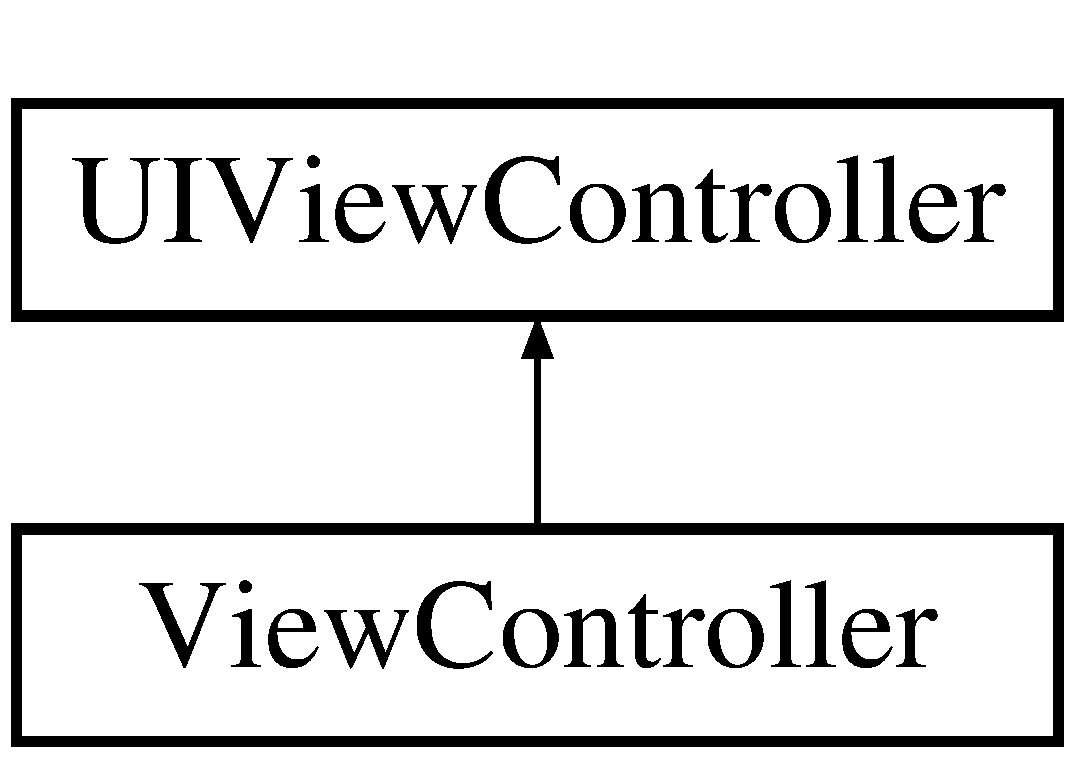
\includegraphics[height=2.000000cm]{interface_view_controller}
\end{center}
\end{figure}
\subsection*{Instance Methods}
\begin{DoxyCompactItemize}
\item 
(I\+B\+Action) -\/ \hyperlink{interface_view_controller_aa54507194ca12f221c64c8626b114945}{change\+Car\+Type\+:}
\end{DoxyCompactItemize}
\subsection*{Properties}
\begin{DoxyCompactItemize}
\item 
\hyperlink{class_car}{Car} $\ast$ \hyperlink{interface_view_controller_aa6bc7a298fc7c20538a2b91787969ae6}{car}
\item 
N\+S\+String $\ast$ \hyperlink{interface_view_controller_a2983301c81b8a147d15df749fab98724}{fun\+Title}
\end{DoxyCompactItemize}


\subsection{Method Documentation}
\hypertarget{interface_view_controller_aa54507194ca12f221c64c8626b114945}{}\index{View\+Controller@{View\+Controller}!change\+Car\+Type\+:@{change\+Car\+Type\+:}}
\index{change\+Car\+Type\+:@{change\+Car\+Type\+:}!View\+Controller@{View\+Controller}}
\subsubsection[{change\+Car\+Type\+:(\+U\+I\+Segmented\+Control $\ast$segmented\+Control)}]{\setlength{\rightskip}{0pt plus 5cm}-\/ (I\+B\+Action) change\+Car\+Type\+: 
\begin{DoxyParamCaption}
\item[{(U\+I\+Segmented\+Control$\ast$)}]{segmented\+Control}
\end{DoxyParamCaption}
}\label{interface_view_controller_aa54507194ca12f221c64c8626b114945}
Change user selection type


\begin{DoxyParams}{Parameters}
{\em segmented\+Control} & U\+I\+Segmented\+Control for change selection\\
\hline
\end{DoxyParams}
Change user selection type


\begin{DoxyParams}{Parameters}
{\em segmented\+Control} & for change selection \\
\hline
\end{DoxyParams}


\subsection{Property Documentation}
\hypertarget{interface_view_controller_aa6bc7a298fc7c20538a2b91787969ae6}{}\index{View\+Controller@{View\+Controller}!car@{car}}
\index{car@{car}!View\+Controller@{View\+Controller}}
\subsubsection[{car}]{\setlength{\rightskip}{0pt plus 5cm}-\/ ({\bf Car}$\ast$) car\hspace{0.3cm}{\ttfamily [read]}, {\ttfamily [write]}, {\ttfamily [nonatomic]}, {\ttfamily [assign]}}\label{interface_view_controller_aa6bc7a298fc7c20538a2b91787969ae6}
\hyperlink{interface_view_controller}{View\+Controller} class object for create new car \hypertarget{interface_view_controller_a2983301c81b8a147d15df749fab98724}{}\index{View\+Controller@{View\+Controller}!fun\+Title@{fun\+Title}}
\index{fun\+Title@{fun\+Title}!View\+Controller@{View\+Controller}}
\subsubsection[{fun\+Title}]{\setlength{\rightskip}{0pt plus 5cm}-\/ (N\+S\+String$\ast$) fun\+Title\hspace{0.3cm}{\ttfamily [read]}, {\ttfamily [write]}, {\ttfamily [nonatomic]}, {\ttfamily [assign]}}\label{interface_view_controller_a2983301c81b8a147d15df749fab98724}
\hyperlink{interface_view_controller}{View\+Controller} class object for create car fun\+Title 

The documentation for this class was generated from the following files\+:\begin{DoxyCompactItemize}
\item 
Documentation\+Examples/View\+Controller.\+h\item 
Documentation\+Examples/View\+Controller.\+m\end{DoxyCompactItemize}

\hypertarget{category_view_controller_07_08}{}\section{View\+Controller() Category Reference}
\label{category_view_controller_07_08}\index{View\+Controller()@{View\+Controller()}}
\subsection*{Properties}
\begin{DoxyCompactItemize}
\item 
I\+B\+Outlet U\+I\+Text\+Field $\ast$ \hyperlink{category_view_controller_07_08_afdb01433312d6957b5642ead0abcc900}{first\+Number\+Field}
\item 
I\+B\+Outlet U\+I\+Text\+Field $\ast$ \hyperlink{category_view_controller_07_08_a08e26ac06941fdcd69176de116478ceb}{second\+Number\+Field}
\item 
I\+B\+Outlet U\+I\+Label $\ast$ \hyperlink{category_view_controller_07_08_a7436e65d71bab732655bcbe6418255b2}{sum\+Label}
\item 
I\+B\+Outlet U\+I\+Label $\ast$ \hyperlink{category_view_controller_07_08_a1ef022914e2412340ecaaa0b3d1e9211}{fun\+Title\+Label}
\end{DoxyCompactItemize}


\subsection{Property Documentation}
\hypertarget{category_view_controller_07_08_afdb01433312d6957b5642ead0abcc900}{}\index{View\+Controller()@{View\+Controller()}!first\+Number\+Field@{first\+Number\+Field}}
\index{first\+Number\+Field@{first\+Number\+Field}!View\+Controller()@{View\+Controller()}}
\subsubsection[{first\+Number\+Field}]{\setlength{\rightskip}{0pt plus 5cm}-\/ (I\+B\+Outlet U\+I\+Text\+Field$\ast$) first\+Number\+Field\hspace{0.3cm}{\ttfamily [read]}, {\ttfamily [write]}, {\ttfamily [nonatomic]}, {\ttfamily [weak]}}\label{category_view_controller_07_08_afdb01433312d6957b5642ead0abcc900}
User First name \hypertarget{category_view_controller_07_08_a1ef022914e2412340ecaaa0b3d1e9211}{}\index{View\+Controller()@{View\+Controller()}!fun\+Title\+Label@{fun\+Title\+Label}}
\index{fun\+Title\+Label@{fun\+Title\+Label}!View\+Controller()@{View\+Controller()}}
\subsubsection[{fun\+Title\+Label}]{\setlength{\rightskip}{0pt plus 5cm}-\/ (I\+B\+Outlet U\+I\+Label$\ast$) fun\+Title\+Label\hspace{0.3cm}{\ttfamily [read]}, {\ttfamily [write]}, {\ttfamily [nonatomic]}, {\ttfamily [weak]}}\label{category_view_controller_07_08_a1ef022914e2412340ecaaa0b3d1e9211}
User fun Title Label \hypertarget{category_view_controller_07_08_a08e26ac06941fdcd69176de116478ceb}{}\index{View\+Controller()@{View\+Controller()}!second\+Number\+Field@{second\+Number\+Field}}
\index{second\+Number\+Field@{second\+Number\+Field}!View\+Controller()@{View\+Controller()}}
\subsubsection[{second\+Number\+Field}]{\setlength{\rightskip}{0pt plus 5cm}-\/ (I\+B\+Outlet U\+I\+Text\+Field$\ast$) second\+Number\+Field\hspace{0.3cm}{\ttfamily [read]}, {\ttfamily [write]}, {\ttfamily [nonatomic]}, {\ttfamily [weak]}}\label{category_view_controller_07_08_a08e26ac06941fdcd69176de116478ceb}
User second Number Field \hypertarget{category_view_controller_07_08_a7436e65d71bab732655bcbe6418255b2}{}\index{View\+Controller()@{View\+Controller()}!sum\+Label@{sum\+Label}}
\index{sum\+Label@{sum\+Label}!View\+Controller()@{View\+Controller()}}
\subsubsection[{sum\+Label}]{\setlength{\rightskip}{0pt plus 5cm}-\/ (I\+B\+Outlet U\+I\+Label$\ast$) sum\+Label\hspace{0.3cm}{\ttfamily [read]}, {\ttfamily [write]}, {\ttfamily [nonatomic]}, {\ttfamily [weak]}}\label{category_view_controller_07_08_a7436e65d71bab732655bcbe6418255b2}
User sum Label 

The documentation for this category was generated from the following file\+:\begin{DoxyCompactItemize}
\item 
Documentation\+Examples/View\+Controller.\+m\end{DoxyCompactItemize}

%--- End generated contents ---

% Index
\backmatter
\newpage
\phantomsection
\clearemptydoublepage
\addcontentsline{toc}{chapter}{Index}
\printindex

\end{document}
